% \lecture{4}{Tue 04 Feb 2020 14:30}{393 Lab 4}

\section{Plots of System response varying $\omega_{0}$, $\zeta$}
The result of varying $\zeta$ is the graph in Figure \ref{fig:varying-zeta}.
\begin{figure}[H]
	\centering
	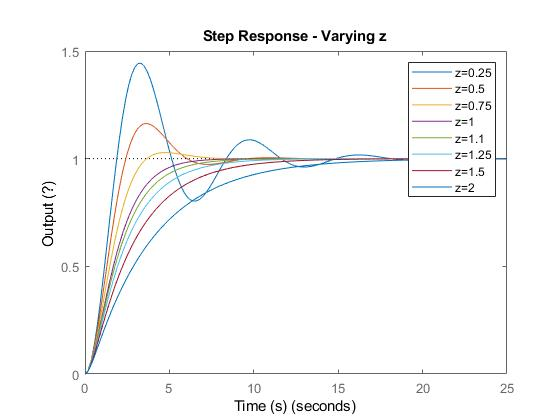
\includegraphics[width=0.8\textwidth]{./figures/lab4_fig1-part4-3-1-z.jpg}
	\caption{A plot of the system response when varying the value of $\zeta$}
	\label{fig:varying-zeta}
\end{figure}
As you can see an increase in $\zeta$ increases the damping of the output, where $\zeta=1$ seems to be close to the critical damping value, $\zeta < 1$ is an underdamped system and $\zeta > 1$ is an overdamped system. 

The result of varying $\omega_{0}$ is seen in Figure \ref{fig:varying-w0}.
\begin{figure}[H]
	\centering
	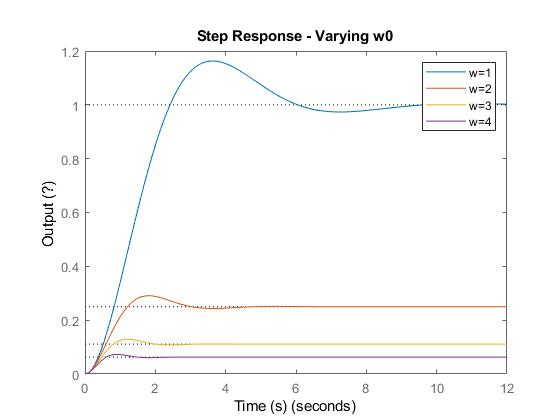
\includegraphics[width=0.8\textwidth]{./figures/lab4_fig2-part4-3-1-w0.jpg}
	\caption{A plot of the system response when varying the value of $\omega _{0}$}
	\label{fig:varying-w0}
\end{figure}
The greater the value of $\omega_{0}$, the smaller the steady-state value of the system. 
\section{Effects of Changing $\alpha$} 

\section{Why Are The Plots The Same?}


\section{System Type Section}

% we can just toss the values in as a screenshot of the excel docs

steady state error for $R_{c} = 5$ : -0.021496
